\documentclass{beamer}
\usepackage{graphicx}
\usepackage{amsmath}
\usepackage{tikz}
\usepackage{hyperref}
\usetheme{Copenhagen}
\title{Variables \& Data Types}
\setbeamertemplate{navigation symbols}{}
\setbeamertemplate{headline}{}
\subtitle{CS 104 MSG 1.1}
\author{Jackson Eshbaugh}
\date{\today}
\institute{Lafayette College}

\AtBeginSection[]{
    \begin{frame}
        \frametitle{Outline}
        \tableofcontents[currentsection, hideothersubsections]
    \end{frame}
}

\begin{document}


\begin{frame}
    \titlepage
\end{frame}

\begin{frame}
    \frametitle{Outline}
    \tableofcontents
\end{frame}

\section{About Me}

\begin{frame}{Jackson Eshbaugh}
    \begin{columns}
        \column{0.5\textwidth}
            \begin{itemize}
                \item Sophomore
                \begin{itemize}
                    \item Computer Science; French
                \end{itemize}
                \only<2>{\item Interested in utilizing computer science to improve other fields of study/research/work
                \begin{itemize}
                    \item i.e., \textit{bioinformatics} or \textit{computational linguistics}
                \end{itemize}}
                \only<3->{\item Aspiring computer science professor, teaching in a holistic way and researching within my wide range of interests.}
                \only<4->{\item \url{jacksoneshbaugh.github.io}}
            \end{itemize}
        \column{0.5\textwidth}
            \includegraphics[width=0.5\textwidth]{JacksonEshbaugh.jpg}
    \end{columns}
\end{frame}

\section{Variables}

\begin{frame}{What is a Variable?}
    \begin{center}
        \only<1->{
            \textbf{\huge Whiteboard it}: \textit{\huge How would you define the term \textbf{variable}?}
        }
        \only<2>{
            \\
            \vspace{2cm}
            \textbf{\Huge $x, y, z \dots$}
        }
    \end{center}
\end{frame}

\begin{frame}[fragile]
    \frametitle{Computer Model}
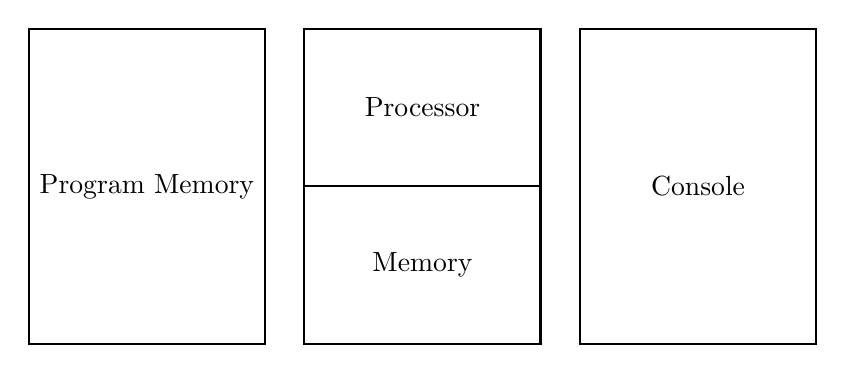
\begin{tikzpicture}
    \draw[thick] (0,0) rectangle (3,4);
    \draw[thick] (3.5,2) rectangle (6.5,4);
    \draw[thick] (3.5,0) rectangle (6.5,2);
    \draw[thick] (7,0) rectangle (10,4);
    \node at (1.5,2) {Program Memory};
    \node at (5,3) {Processor};
    \node at (5,1) {Memory};
    \node at (8.5,2) {Console};
\end{tikzpicture}
\begin{itemize}
    \item Recall this model of the computer from class.
\end{itemize}
\end{frame}

\begin{frame}[fragile]
    \frametitle{Computer Model}
    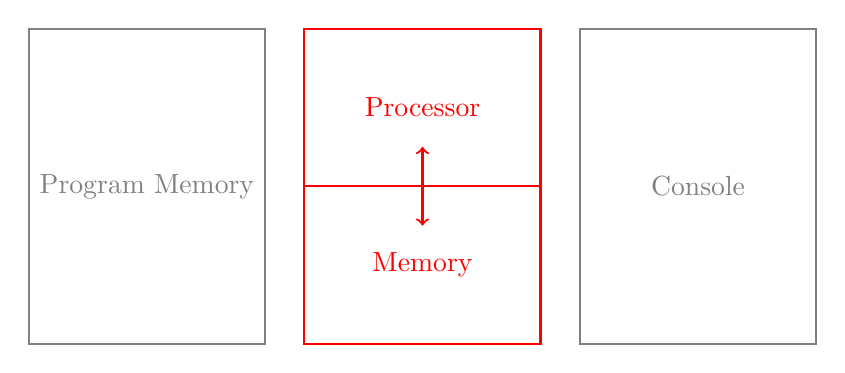
\begin{tikzpicture}
        \draw[thick, gray] (0,0) rectangle (3,4);
        \draw[thick, red] (3.5,2) rectangle (6.5,4);
        \draw[thick, red] (3.5,0) rectangle (6.5,2);
        \draw[thick, gray] (7,0) rectangle (10,4);
        \node[gray] at (1.5,2) {Program Memory};
        \node[red] at (5,3) {Processor};
        \node[red] at (5,1) {Memory};
        \node[gray] at (8.5,2) {Console};
        \draw[<->, thick, red] (5,1.5) -- (5,2.5);
    \end{tikzpicture}
\begin{itemize}
    \item Variables deal with the memory (and the processor).
\end{itemize}
\end{frame}

\begin{frame}[fragile]
    \frametitle{Variable Example}
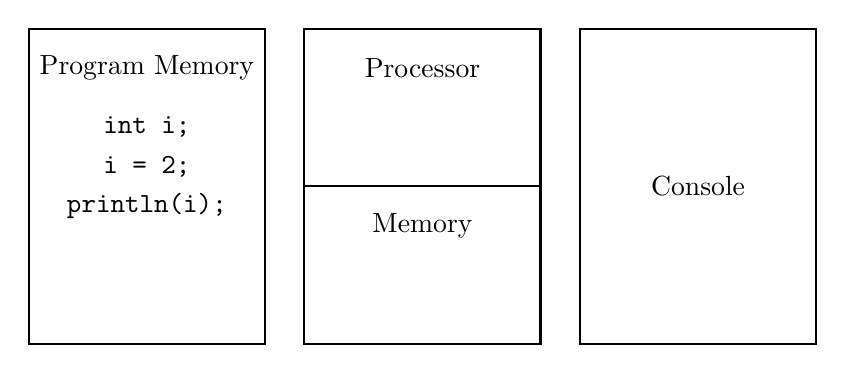
\begin{tikzpicture}
    \draw[thick] (0,0) rectangle (3,4);
    \draw[thick] (3.5,2) rectangle (6.5,4);
    \draw[thick] (3.5,0) rectangle (6.5,2);
    \draw[thick] (7,0) rectangle (10,4);
    \node at (1.5,3.5) {Program Memory};
    \node at (1.5,2.75) {\texttt{int i;}};
    \node at (1.5,2.25) {\texttt{i = 2;}};
    \node at (1.5,1.75) {\texttt{println(i);}};
    \node at (5,3.5) {Processor};
    \node at (5,1.5) {Memory};
    \node at (8.5,2) {Console};
\end{tikzpicture}
\begin{itemize}
        \item Variables are stored in memory.
\end{itemize}
\end{frame}

\begin{frame}
    \frametitle{Data Types}
    \begin{itemize}
        \item Computers are mathematical devices at their cores.
    \end{itemize}
\end{frame}

\begin{frame}
    \frametitle{Data Types}
    \only<1->{
        \begin{itemize}
            \item Computers are mathematical devices at their cores.
            \item This implies that all data we encounter must be numerical at its core.
        \end{itemize}
    }
    \only<2>{
        \begin{center}
            \textbf{\Huge $\Rightarrow$ Enter \textit{data types}.}
        \end{center}
    }
\end{frame}

\section{Data Types}

\begin{frame}
    \frametitle{Data Types}
    \begin{itemize}
        \item Data types define the type of data a variable can hold.
        \item In other words, the data type of a variable is used to interpret the stored numerical value.
    \end{itemize}
\end{frame}

\begin{frame}
    \frametitle{Data Type Examples}
    \begin{table}[h]
        \centering
        \begin{tabular}{|c|c|}
            \hline
                            \textbf{Data Type} & \textbf{Represents} \\ \hline
                            \texttt{int} & \hspace{5cm} \\ \hline
                            \texttt{float} & \hspace{5cm} \\ \hline
                            \texttt{double} & \hspace{5cm} \\ \hline
                            \texttt{char} & \hspace{5cm} \\ \hline
                            \texttt{boolean} & \hspace{5cm} \\ \hline
                            \texttt{String} & \hspace{5cm} \\ \hline
                        \end{tabular}
        \caption{Data Types and What They Represent}
        \label{tab:data_types}
    \end{table}
\end{frame}

\section{Expressions}

\begin{frame}
    \frametitle{Operators}
    \begin{itemize}
        \only<1->{
            \item Operators operate on operands—variables or literal numbers.
        }
        \only<2->{
            \item \texttt{+} — addition
        }

        \only<3->{
            \item \texttt{-} — subtraction
        }

        \only<4->{
            \item \texttt{*} — multiplication
        }

        \only<5->{
            \item \texttt{/} — division
        }

        \only<6->{
            \item \texttt{\%} — modulus
        }
    \end{itemize}
\end{frame}

\begin{frame}[fragile]
    \frametitle{Operator Examples}

    What will the following code output? What will the memory look like after execution?
    \begin{verbatim}
        int i = 12;
        int j = 7;
        println(3 * x);
        int k = i + j - 2;
        println(k);

        int l = 3;
    \end{verbatim}
    \only<1> {\hspace{1.5cm} \texttt{println(l / 2);}}
    \only<2>{\hspace{1.5cm} \color{red}\texttt{println(l / 2);}}
\end{frame}

\begin{frame}
    \frametitle{Dangers of Division}

    \begin{itemize}
        \item Depending on the data type, \texttt{a / b} yields different results.
        \only<2->{
            \item If \textit{both} \texttt{a} and \texttt{b} are integer or other non-decimal numerical types, \texttt{a / b} yields an integer value, \textbf{truncating the decimal.}
        }
        \only<3-> {
            \item If \textit{either} \texttt{a} or \texttt{b} are floating point types (\texttt{float}, \texttt{double}), then \texttt{a / b} yields a float. 
        }
    \end{itemize}
\end{frame}

\begin{frame}[fragile]
    \frametitle{Modulus}

    \begin{itemize}
        \item You've all been using modulus for most of your life: \only<2->{ \textbf{to tell time}! }
    \end{itemize}

\end{frame}

\begin{frame}[fragile]
    \frametitle{Modulus}

    \begin{itemize}
        \item You've all been using modulus for most of your life: \textbf{to tell time}!
    \end{itemize}

    \begin{verbatim}
        15 % 5 =                   8 % 3 =


        
        3 % 2 =                   12 % 15 =


\end{verbatim}

\end{frame}

\section{Q \& A}
\begin{frame}
    \centering \textbf{Q \& A}: If you need help, let me know. Let’s try to help each other out.
\end{frame}

\end{document}
